\documentclass{article}
\usepackage[pdftex]{graphicx}
\usepackage{wrapfig}
\usepackage{enumerate}
\usepackage{hyperref}
\usepackage{fullpage}
\usepackage{cite}

\begin{document}

\title{CSE550 Problem Set 3: Performance Evaluation of Least Common Ancestors on Spark}
\author{Vincent Lee, Shumo Chu}
\date{\today}

\maketitle

\tableofcontents

%%%%%%%%%%%%%%%%%%%%%%%%%%%%%%%%%%%%%%%%%%%%%%%%%%%%%%%%%%%%%%%%%%%%%%%%%%%%%%
% Intro
%%%%%%%%%%%%%%%%%%%%%%%%%%%%%%%%%%%%%%%%%%%%%%%%%%%%%%%%%%%%%%%%%%%%%%%%%%%%%%

\section{Introduction}
\label{sec:intro}
The Least Common Ancestor (LCA) algorithm is a method of determining a which node in the graph minimize a distance function given two other nodes in a directed acyclic graph (DAG).
Given two papers $p_1$ and $p_2$, we want to find the LCA of the two papers defined $LCA(p_1, p_2)$ if it exists.
A common ancestor is defined as any paper $p_i$ that has a path to both $p_1$ and $p_2$.
Note that the set $S(p_1, p_2)$ denoting the set of common ancestors of $p_1$ and $p_2$ can be arbitrarily large or empty.
The least common ancestor is defined to be paper $p_{lca}$ in $S(p_1, p_2)$ which minimizes a cost function.
Of course if the set $S(p_1, p_2)$ is empty, no such LCA exists for the two papers.
The cost function for any paper $p_i \in S(p_1, p_2)$ is defined as the maximum of the distances between $p_1$ and $p_{lca}$, and $p_2$ and $p_{lca}$ where each edge in the directed graph has equal weight.
Each paper also contains two attributes used to help break ties between equidistant candidates in the graph: a publication year, and unique paper identifier.
Should multiple papers have equal cost by the distance metric, the year of publication is used to break a tie where a lower year of publication minimizes this secondary cost function.
Should multiple papers have both equal distance cost and year of publication, the unique paper identification is used to determine the LCA.
The paper with the least unique identification is chosen as the LCA.

In this project we implement the LCA algorithm for a DAG of paper citations; citations graphs are acyclic as paper citations are causal.
We implement the LCA problem in Spark on top of Amazon's EC2 platform.

\section{Algorithm and Implementation}
Our algorithm contains two parts: the first part is to compute the shorted path
from vertices in to citation graph to seed vertices, and the second part is to 
find the lowest common accestors for any pairs of papers in the seed set.

\subsection{Part 1: Parallel Bellman-Ford Algorithm in Spark}
We use a parallel version of Bellman-Ford algorithm and implemented it in
Spark. Bellman-Ford is an ideal choice because: 

\begin{enumerate}
    \item The citation graph does not contain any negetive cycles 
    thus Bellman-Ford algorithm is correct.
    \item Bellman-Ford algorithm is easily parallelized.
\end{enumerate}

We store the graph in the form of edges in a RDD and initialize the distances
from the seed vertices to themselves as $0$. Then in each iteration, we join
the distances RDD with the edges in the graph and only keep the shortest
distances of any paper to one of the seed vertices. This iterative process will
be ended if there is no new distance computed.

\subsection{Part 2: Lowest Accestor Computation}
For part 1, we have distances from any seed vertex to its reachable vertices. 
We then join the $(paper, year)$ data with this distance data to attach the 
year published to the distance RDD. Then the distance RDD with the year data 
is self joined on its paper id to get comman ancestor for each pairs of seeded 
vertices. At last, a communitive reduce function is implemented according to
the lowest comman accestor criteria described in Section~\ref{sec:intro}.

\section{Running Our Code}

Our repository is composed of a top level Makefile which is used to launch and bring up the Spark cluster.
In order to use the script, the EC2 sparks scripts from the Spark distribution must be added to the $PATH$ variable.
By running $make launch$, our script will bring up a new Spark cluster on EC2.
This launch script occassionally times out and gives up if the EC2 cluster does not finish its self-checks in time.
Once the cluster is up, we can stop it using $make stop$ and resume it using $make resume$.
To log in, we use $make login$ which opens an ssh session with our cluster.

Once logged into our cluster, we configure the $PATH$ variable to contain the binaries for $spark-submit$.
We also clone our project repository or SCP the Spark application to some deployable location on the cluster.
Our $src$ directory, contains a Makefile that contains a $test$ target defined in $test.py$ which can be used as a sanity check to verify that the Spark cluster was properly resumed or intialized.
This $test$ target executes the example Spark job from the assignment specification that counts the number of times the string ``12'' occurs in the cites.csv file.
The default $all$ target in our Makefile launches our LCA application defined in $lca.py$.
Launching the LCA application will execute the specified algorithm across all nodes available on the cluster on the original data set.
The source for the LCA Spark application is located in $lca.py$.

When we are done with our cluster, we issue a $make destroy$ command at the top level Makefile to tell EC2 to bring down and destroy our cluster.

\section{Performance Evaluation}

\paragraph{Dataset and Experiment Settings}
We use two datasets, one is the citation graph in the schema of 
$(paper, cited paper)$, the other is the meta data of each paper, in the schema
of $(paper, year)$. Citation graph contains $8,227,538$ citations. Meta data 
of paper contains year information for $1,787,349$ papers.

We deploy a spark cluster with $20$ Amazon EC2 instances. One instance is used
as master node, the other $19$ of the instances are used as slave nodes. 
Each EC2 instance is a $m3.large$ type instance with single CPU and $3.75$ GB
RAM.

\subsection{Raw Performance}

To analyze the scalability of our implementation and platform, we evaluate the latency of a single query on a varying size dataset.

\begin{figure}
\centering
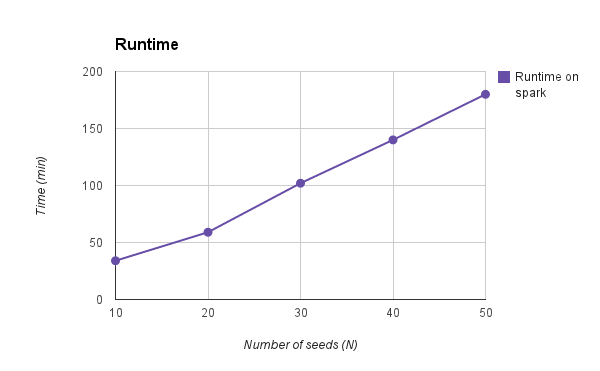
\includegraphics[width=0.7\textwidth]{runtime.png}
\caption{LCA compuatation time with increasing seed set size}
\label{latency_scaling}
\end{figure}

Figure ~\ref{latency_scaling} shows the compuation time with 
increasing number of seeded vertices.
As expected, we see an increase in the query latency with respect to 
increasing data set size. The runtime of the program is dominated by the 
shortest path computation time. And that part of cost increase near linearly 
as the number of seeded vertices increases. So we can see that the computation 
time increases almost linearly as the number of seeded vertices increases.


\begin{figure}
\centering

%%%%%%%%%%%%%%%%%%%%%%%%%%%%%%%%%%%%%%%%%%%%%%%%%%%%%%%%%%%%%%%%%%%%%%%%%%
% @SHUMO TODO - add the graph
%%%%%%%%%%%%%%%%%%%%%%%%%%%%%%%%%%%%%%%%%%%%%%%%%%%%%%%%%%%%%%%%%%%%%%%%%%

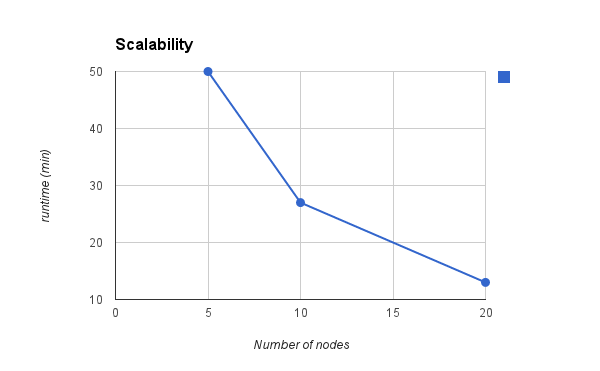
\includegraphics[width=0.7\textwidth]{scalability.png}

\caption{LCA query latency with increasing number of cluster nodes}
\label{node_scaling}
\end{figure}

Figure ~\ref{node_scaling} shows the query latency scaling with respect to the number of nodes in the Amazon EC2 cluster instance.
As expected, we see a decrease in query latency time for a fixed data set with more nodes due to additional parallelism.

We note that the performance of the system is composed of roughly two phases: building the graph and actual graph traversal time.

Since our primary parallelization optimizations occur in the graph traversal when searching for the LCA, we expect that simply throwing additional cluster nodes at our application will be constrained by Amdahl's limits in terms of  perfspeed up.
This is evident in Figure ~\ref{node_scaling} where we see asymptotic gains in improvement. 
If the performance was entirely composed of entirely parallel computation, we should see an asymptotic performance improvement towards zero latency.
As shown in the performance curve, this is not the case due to serialized portions of the algorithm and other overheads such as network communication and memory access.

The latency scalability we observe is not surprising as Amdahl's law would require we improve the serialized portions of the algorithm in order to achieve truly linear speed up.
However, since our application is not embarrassingly parallel, the scalability numbers we observe from our experiements are fairly reasonable.

\begin{figure}
    \centering
        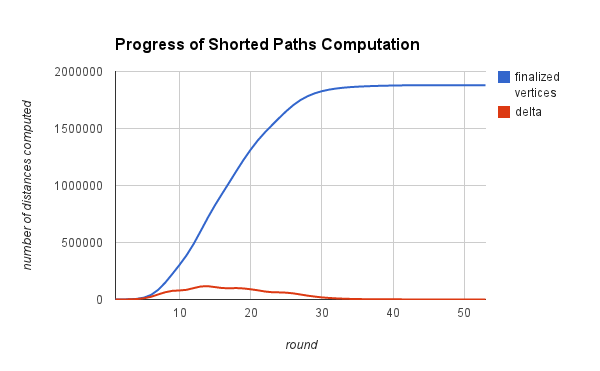
\includegraphics[width=0.8\textwidth]{sssp.png}
    \caption{shortest path progress in each round}
    \label{fig:shortest_path}
\end{figure}

Figure~\ref{fig:shortest_path} shows the progress for each round BFS, we can
clearly see there is a long tail as the search is going to end.

\subsection{Throughput Per Hour}

While query latency is an important metric of performance for many applications, we believe that most applications of the LCA algorithm are not latency sensitive; in other words, latency is an incomplete metric of implementation performance.
One could conceivably build the citation graph, pre-compute all of the LCAs and then cache the results for incoming queries.
This would only require a one time cost of building the index to service arbitrarily many queries; since the LCA index can be built offline, throughput is arguably a more important factor than latency.
Thus to get an idea of how our implementation performs on the throughput axis, we measure the throughput per hour of our system.

We measure the throughput and scalability of our implementation, we tried to determine the number LCAs for a given dataset size N we were able to compute in an hour.

\begin{figure}
    \centering
    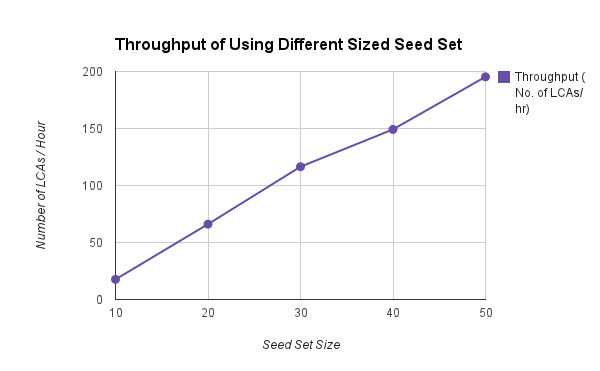
\includegraphics[width=0.7\textwidth]{throughput.png}
    \caption{Throughput using different seed size}
    \label{fig:throughput}
\end{figure}

\begin{table}[h]
    \begin{tabular}{|l|l|l|}
    \hline
    No. of Seeds  & No. of LCAs & Throughput (LCAs/Hr) \\ \hline
    10 & 10          & 17.647               \\ \hline
    20 & 65          & 66.102               \\ \hline
    30 & 198         & 116.471              \\ \hline
    40 & 373         & 149.2                \\ \hline
    50 & 586         & 195.333              \\ \hline
    \end{tabular}
\end{table}


\section{Analytics Platform Evaluation}

The big data analytics platform we used for this project was Apache Spark.
This choice of platform was both a good and bad fit as the LCA algorithm has portions of the algorithm which lend themselves well to the Spark API well and some portions do not.
For instance, when performing the graph traversal, it may have been much easier from a programmability and execution model aspect to use GraphLab's optimized single source shortest path API.
However, the Spark execution and programming model allows more flexible parallelization by offering automatically parallelizable arbitrary lambda expressions.
We argue that this flexibility is more important than being restricted to GraphLab's API.
Thus we conclude Spark was a mediocre fit for highly optimized graph travesral operations, but a good fit for portions of the algorithm that have no direct GraphLab API mapping such as the JOIN operations we need to execute when computing the cost function of LCA candidates.

Aside from performance, there were many problems just with getting the platform to run in the EC2 infrastructure properly and get Spark to deploy properly.
While for an Apache project, Spark appears to have an acceptable amount of documentation, we found the any sort of debugging or trouble shooting infrastructure help was impossibly difficult to find or insufficiently documented on forums.
Thus we spent a vast majority of our time attempting to deploy and figure out how to properly use Spark's arcane API.
In particular the EC2 deployment scripts often resulted in unintelligible error messages when not configured properly.
The Spark documentation, while straightforward, was insufficient in communicating how to use some of Spark's API to efficiently implement the algorithm.
Furthermore, we experienced random terminations of our EC2 instance Spark clusters while running our experiments, and Spark runtime application crashes which were not properly documented.
Finally, we also ran in to problems when resuming stopped instances of our cluster.
There were a few instances where attempts to resume the cluster would fail with an error claiming that the cluster instances could not open communication channels with each other and the resume directive would just give up.
These deployment issues combined with the insufficiently documented Spark API made implementing and deploying our application much more frustrating then the Paxos assignment.

\end{document}
